\documentclass{standalone}
\usepackage{pgfplots}
\usepackage{xcolor}
\pgfplotsset{compat=1.17}

% Auburn colors
\definecolor{auburnorange}{RGB}{232, 119, 34}
\definecolor{auburnblue}{RGB}{12, 35, 64}

\begin{document}
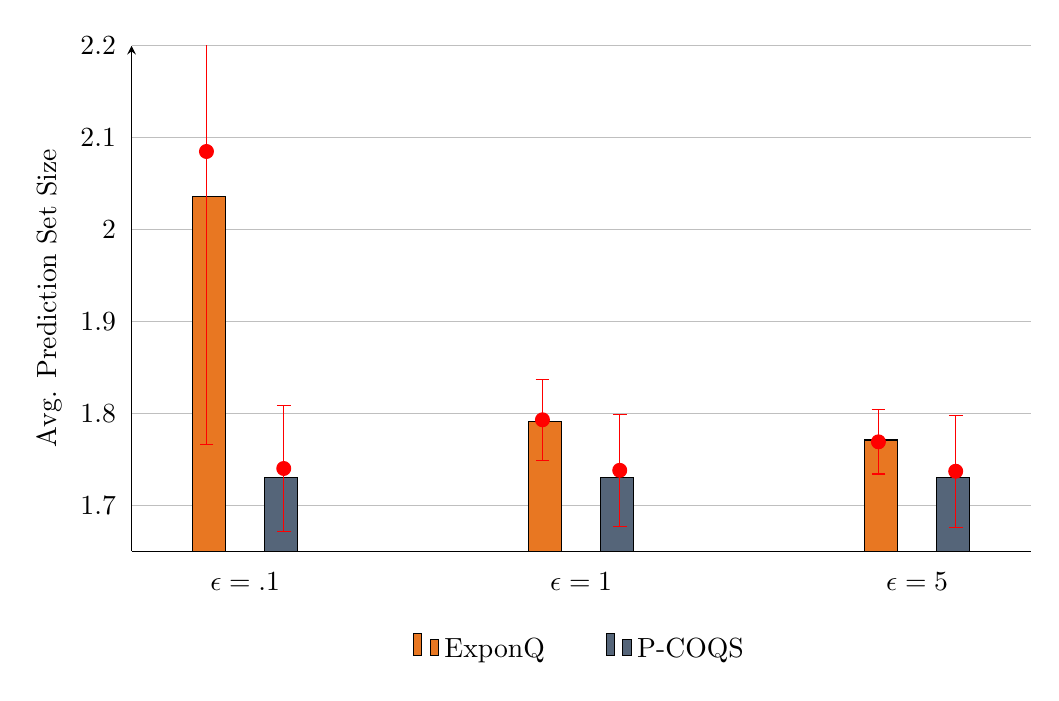
\begin{tikzpicture}
\begin{axis}[
    ybar,
    bar width=12pt,
    enlargelimits=0.1,
    ymin=1.65, ymax=2.2,
    ylabel={Avg. Prediction Set Size},
    xtick={1,2,3},
    xticklabels={$\epsilon=.1$, $\epsilon = 1$, $\epsilon=5$},
    legend style={
        at={(0.5,-0.15)},
        anchor=north,
        legend columns=2,
        /tikz/every even column/.append style={column sep=2em},
        draw=none
    },
    ymajorgrids=true,
    axis x line*=bottom,
    axis y line=left,
    tick style={draw=none},
    width=13cm,
    height=8cm,
]

% --- ExponQ median bars ---
\addplot+[
    draw=black,
    fill=auburnorange,
] coordinates {
    (0.95, 2.036) 
    (1.95, 1.791)
    (2.95, 1.771)
};

% --- P-COQS median bars ---
\addplot+[
    draw=black,
    fill=auburnblue!70,
] coordinates {
    (1.05, 1.730)
    (2.05, 1.730)
    (3.05, 1.730)
};

% --- Mean red points with 2×SD error bars ---
\addplot+[
    color=red,
    only marks,
    mark=*,
    mark size=2.5pt,
    error bars/.cd,
    y dir=both,
    y explicit,
] coordinates {
    (0.885, 2.085) +- (0, 0.319)
    (1.115, 1.740) +- (0, 0.069)
    (1.885, 1.793) +- (0, 0.044)
    (2.115, 1.738) +- (0, 0.061)
    (2.885, 1.769) +- (0, 0.035)
    (3.115, 1.737) +- (0, 0.061)
};

\legend{ExponQ\hspace{5em}, P-COQS}
\end{axis}
\end{tikzpicture}
\end{document}
